\section{地方性的重要节日}

\subsection{慕尼黑啤酒节}

慕尼黑啤酒节又称“十月节”(Oktoberfest),起源于1810年10月12日,因在这个节日期间主要的饮料是啤酒,所以人们习惯性地称其为啤酒节。每年九月末到十月初在德国的慕尼黑举行,持续两周,到十月的第一个星期天为止,是慕尼黑一年中最盛大的活动。慕尼黑啤酒节与英国伦敦啤酒节、美国丹佛啤酒节并称世界最具盛名的三大啤酒节。慕尼黑啤酒节在一个叫做“Theresienwiese”的地方,巴伐利亚方言简称为“Wiesn”,意为牧场。每年大约有六百万人参与其中。 

\subsubsection{起源及历史沿革}

1810年10月12日,巴伐利亚的王储路德维希与萨克森王国的特蕾泽·夏洛特·露易丝公主举行盛大的婚礼。王储的父亲约瑟夫决定为他儿子的婚礼举行为期两天的庆祝活动。为了表示国王对其臣民的恩典,在这两天的活动中,在慕尼黑有4个地方向全体平民免费供应饭菜和饮料。王国的骑兵卫队还在慕尼黑西南的一个大草坪上举行赛马活动和射击比赛,以示助兴。为了纪念这个节日,参赛的官兵请求国王用新娘特蕾泽的名字来命名这个草坪,从那时起这个草坪就叫“特蕾泽”草地。由于庆典给人们留下了深刻的印象,所以人们建议1811年再搞一次全民性的活动。以后就每年举办一次。这就是十月节的起源。

从1810年到2014年为止,慕尼黑啤酒节有204年的历史。其间因第一次世界大战停办5年;第二次世界大战停办7年。自1946年以来节日规模越办越大,从而真正成了一个盛大的民间节日。

\subsubsection{风俗活动}
\begin{enumerate}
    
\item 开幕仪式

每逢十月节开幕那天,要举行盛大的开幕式和由各大啤酒厂组织的五彩缤纷的游行。开幕式在一个临时搭起的大帐篷里由慕尼黑市市长主持。中午12时,在12响礼炮声和音乐声中,市长用一柄木槌把黄铜龙头敲进一个大啤酒桶内,然后拧开龙头,把啤酒放出来,盛在特制的大啤酒杯中。市长饮下这第一杯,著名的十月节便正式开始了。

\item 盛装巡游 

每年啤酒节的第一个周日,来自全德国各个州的人们穿上富有特色的民族服装,演奏音乐,浩浩荡荡的穿过慕尼黑的市中心,最后来到啤酒节的现场Theresienwiese。人们把自己打扮成古代衣着考究的贵族公爵,身披绫罗绸缎的王妃贵妇,驾着鲜花装扮的古典马车,也有不少人很朴实的穿着农民过节穿的衣服。参加的人从老到少,有家庭妇女,中学生,连幼儿园小朋友都有。扮演的人物也是丰富多彩,有阿尔卑斯山下的牧童,莱茵河畔的磨房主,到科隆教堂的修女,北德普鲁士的老翁。

\item 啤酒帐篷

为了招徕本国顾客和接待来慕尼黑旅游的外国客人,慕尼黑的八大啤酒厂在节前就在特蕾泽大广场上搭起巨大的啤酒大篷,德语里称“Bierzelten”,比一般的帐篷装修更大也更豪华。每个帐篷里放有长条木桌和板凳,大篷的一端还有一个临时舞台,由民间乐队演奏欢乐的民间乐曲。帐篷一般可容纳三四千人,最大的有7000个座位。

每一个啤酒棚一般都只提供一个酿酒厂的啤酒,为了突出自己的与众不同,每个啤酒厂都把自己的那个啤酒棚修建的富有特色而舒适气派。啤酒棚外部的装修标新立异,但内部大多都是一个格局,可以坐二十人的长条木桌椅排排摆开,会场中心是被鲜花和灯光装扮一新的高高的表演舞台,棚顶装饰着巨幅的绸缎和编织的花环,有的啤酒棚还设两层,楼上便是"雅座"。各帐篷里都由身穿巴伐利亚民族服装的女服务员给顾客送酒。
\end{enumerate}

\subsection{泼水节}

泼水节是中国傣族以及东南亚泰语民族的传统节日。一般在农历的四月中旬,持续3到7天. 期间,大家用纯净的清水相互泼洒,祈求洗去过去一年的不顺。同时泼水节是展现傣族的水文化、音乐舞蹈文化、饮食文化、服饰文化等传统文化的综合舞台。

\begin{figure}
    \centering
    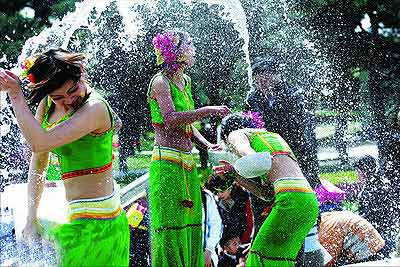
\includegraphics[width=0.6\linewidth]{poshui-fest}
    \caption{云南泼水节}
\end{figure}
泼水节最早起源于公元5世纪的波斯,经印度传入中国云南。关于泼水节的来历有一个古老的传说,从前有一个无恶不作的魔王霸占了美丽富饶的西双版纳,并抢来七位美丽的姑娘做他的妻子。姑娘们满怀仇恨,合计着如何杀死魔王。一天夜里,年纪最小的姑娘把魔王灌得大醉,使他吐露自己致命的弱点。原来这个魔王怕用他的头发勒住自己的脖子。小姑娘拔下魔王一根头发,勒住他的脖子。果然,魔王的头就掉了下来,变成一团火球,滚到哪里,邪火就蔓延到哪里。竹楼被烧毁,庄稼被烧焦。为了扑灭火,小姑娘揪住了魔王的头,其他六位姑娘不停地向上面泼水,终于在六月把火扑灭了。从此,便有了泼水的习俗。在泼水节当天既有丰富的活动,也有美丽的爱情。这一天男女老少共聚村中广场,围成一圈,和着鼓点翩翩起舞,边唱边跳。未婚的青年男女们在草坪上各站一排,先由姑娘把手里的包掷给中意的小伙子,小伙子再掷给姑娘。小伙子若是接不住姑娘丢来的花包,就得把事先准备好的鲜花插在姑娘的头上,姑娘若是接不着小伙子丢来的包,就得把鲜花插到小伙子的胸前,彼此来传达自己的爱慕之情。。同时泼水节还是加强西双版纳全州各族人民大团结的重要纽带,对西双版纳与东南亚各国友好合作交流,对促进全州社会经济文化的发展起到了积极作用。因此2006年5月20日,该民俗经国务院批准列入中国第一批国家级非物质文化遗产名录。